% ------------------------------------------------------------------------------
% TYPO3 CMS 8.3 - What's New - Chapter "In-Depth Changes" (English Version)
%
% @author	Patrick Lobacher <patrick@lobacher.de> and Michael Schams <schams.net>
% @license	Creative Commons BY-NC-SA 3.0
% @link		http://typo3.org/download/release-notes/whats-new/
% @language	English
% ------------------------------------------------------------------------------
% LTXE-CHAPTER-UID:		5ebcecbe-66abfa57-cf38bc00-aa637965
% LTXE-CHAPTER-NAME:	In-Depth Changes
% ------------------------------------------------------------------------------

\section{Cambios en Profundidad}
\begin{frame}[fragile]
	\frametitle{Cambios en Profundidad}

	\begin{center}\huge{Capítulo 3:}\end{center}
	\begin{center}\huge{\color{typo3darkgrey}\textbf{Cambios en Profundidad}}\end{center}

\end{frame}

% ------------------------------------------------------------------------------
% LTXE-SLIDE-START
% LTXE-SLIDE-UID:		b744dad0-9f9864e9-2bd62e7e-02985fbe
% LTXE-SLIDE-ORIGIN:	bd33b29d-c20d1765-f923f78e-43bfb0bf English
% LTXE-SLIDE-TITLE:		Feature #74365: Add Linkservice for Unified Referencing Syntax (1)
% LTXE-SLIDE-REFERENCE:	Feature-74365-LinkServiceForUnifiedReferencingSyntax.rst
% ------------------------------------------------------------------------------
\begin{frame}[fragile]
	\frametitle{Cambios en Profundidad}
	\framesubtitle{Añadir Linkservice para Sintaxis de Referenciado Unificada (1)}

	\begin{itemize}

		\item Recursos dentro de TYPO3 han sido referenciados usando múltiples y diferentes formas de sintaxis en el pasado.

		\item TYPO3 ahora soporta un modo moderno y a prueba de futuro de referenciar recursos usando una sintaxis
			extensible y expresiva que es sencilla de entender.

		\item Las siguientes diapositivas explican la sintaxis usando el siguiente enlace de página simple:

			\begin{lstlisting}
				t3://page?uid=13&campaignCode=ABC123
			\end{lstlisting}

	\end{itemize}

\end{frame}

% ------------------------------------------------------------------------------
% LTXE-SLIDE-START
% LTXE-SLIDE-UID:		b6b5f911-1b9701d3-7b8e4eab-6257c954
% LTXE-SLIDE-ORIGIN:	95f9a663-ea2155a1-5635728b-77a8995c English
% LTXE-SLIDE-TITLE:		Feature #74365: Add Linkservice for Unified Referencing Syntax (2)
% LTXE-SLIDE-REFERENCE:	Feature-74365-LinkServiceForUnifiedReferencingSyntax.rst
% ------------------------------------------------------------------------------
\begin{frame}[fragile]
	\frametitle{Cambios en Profundidad}
	\framesubtitle{Añadir Linkservice para Sintaxis de Referenciado Unificada (2)}

	\begin{itemize}

		\item La sintaxis consiste en tres partes:

			\begin{itemize}

				\item Espacio de nombres (\texttt{t3://})\newline
		   			El espacio de nombres es fijado a \texttt{t3://} para asegurar que el "LinkService" es ejecutado para pasear la URN.
					\newline
				\item Clave de manejador de recurso (\texttt{page})\newline
   					La clave de manejador de recurso es una lista de manejadores disponibles en TYPO3.
					En el momento actual existen los siguientes manejadores: \texttt{page}, \texttt{file} and \texttt{folder}.\newline
					Se pueden configurar más claves en un vector asociativo, donde la clave es el manejador y el valor
					es una clase implementando el LinkHandlerInterface:\newline
					\texttt{\$TYPO3\_CONF\_VARS['SYS']['linkHandler']}

			\end{itemize}

	\end{itemize}

\end{frame}

% ------------------------------------------------------------------------------
% LTXE-SLIDE-START
% LTXE-SLIDE-UID:		7984813b-fb2b3d13-752a7fd7-15e1d06b
% LTXE-SLIDE-ORIGIN:	77a8995c-ea2155a1-95f9a663-5635728b English
% LTXE-SLIDE-TITLE:		Feature #74365: Add Linkservice for Unified Referencing Syntax (3)
% LTXE-SLIDE-REFERENCE:	Feature-74365-LinkServiceForUnifiedReferencingSyntax.rst
% ------------------------------------------------------------------------------
\begin{frame}[fragile]
	\frametitle{Cambios en Profundidad}
	\framesubtitle{Añadir Linkservice para Sintaxis de Referenciado Unificada (3)}

	\begin{itemize}

		\item ... y la tercera parte:

			\begin{itemize}

				\item Parámetros de recurso (\texttt{?uid=13\&campaignCode=ABC123})\newline
					Éstos son los parámetros de identificación específicos que son usados por cualquier manejador.
					Note que éstos pueden acarrear parámetros adicionales para configurar el comportamiento de cualquier manejador.

			\end{itemize}

	\end{itemize}

\end{frame}

% ------------------------------------------------------------------------------
% LTXE-SLIDE-START
% LTXE-SLIDE-UID:		2e9ee046-c3c1a9aa-d24aae82-4acd47c4
% LTXE-SLIDE-ORIGIN:	af8e73a4-2b315873-bb6e55e4-c0cd82b5 English
% LTXE-SLIDE-TITLE:		#76008 and #76458: DebuggerUtility::var_dump (1)
% LTXE-SLIDE-REFERENCE:	Feature-76008-PropertyVisibilityToDebuggerUtilityvar_dump.rst
% LTXE-SLIDE-REFERENCE:	Feature-76458-LetDebuggerUtilityRenderClosures.rst
% ------------------------------------------------------------------------------
\begin{frame}[fragile]
	\frametitle{Cambios en Profundidad}
	\framesubtitle{\texttt{DebuggerUtility::var\_dump} (1)}

	\begin{itemize}

		\item La información de la propiedad visibility ha sido añadida a \texttt{DebuggerUtility::var\_dump()}
			\newline
			para cada propiedad de objeto en el dump

		\item Si una firma es parte del objeto de depuración, el código fuente de la firma es renderizado, también

	\end{itemize}

	\tabto{0.75cm}\textit{Ver ejemplo en la siguiente diapositiva}

\end{frame}

% ------------------------------------------------------------------------------
% LTXE-SLIDE-START
% LTXE-SLIDE-UID:		278b6e97-92e701c6-2dc704e2-17e52b66
% LTXE-SLIDE-ORIGIN:	bb6e55e4-2b315873-c0cd82b5-af8e73a4 English
% LTXE-SLIDE-TITLE:		#76008 and #76458: DebuggerUtility::var_dump (2)
% LTXE-SLIDE-REFERENCE:	Feature-76008-PropertyVisibilityToDebuggerUtilityvar_dump.rst
% LTXE-SLIDE-REFERENCE:	Feature-76458-LetDebuggerUtilityRenderClosures.rst
% ------------------------------------------------------------------------------
\begin{frame}[fragile]
	\frametitle{Cambios en Profundidad}
	\framesubtitle{\texttt{DebuggerUtility::var\_dump} (2)}

	\begin{figure}
		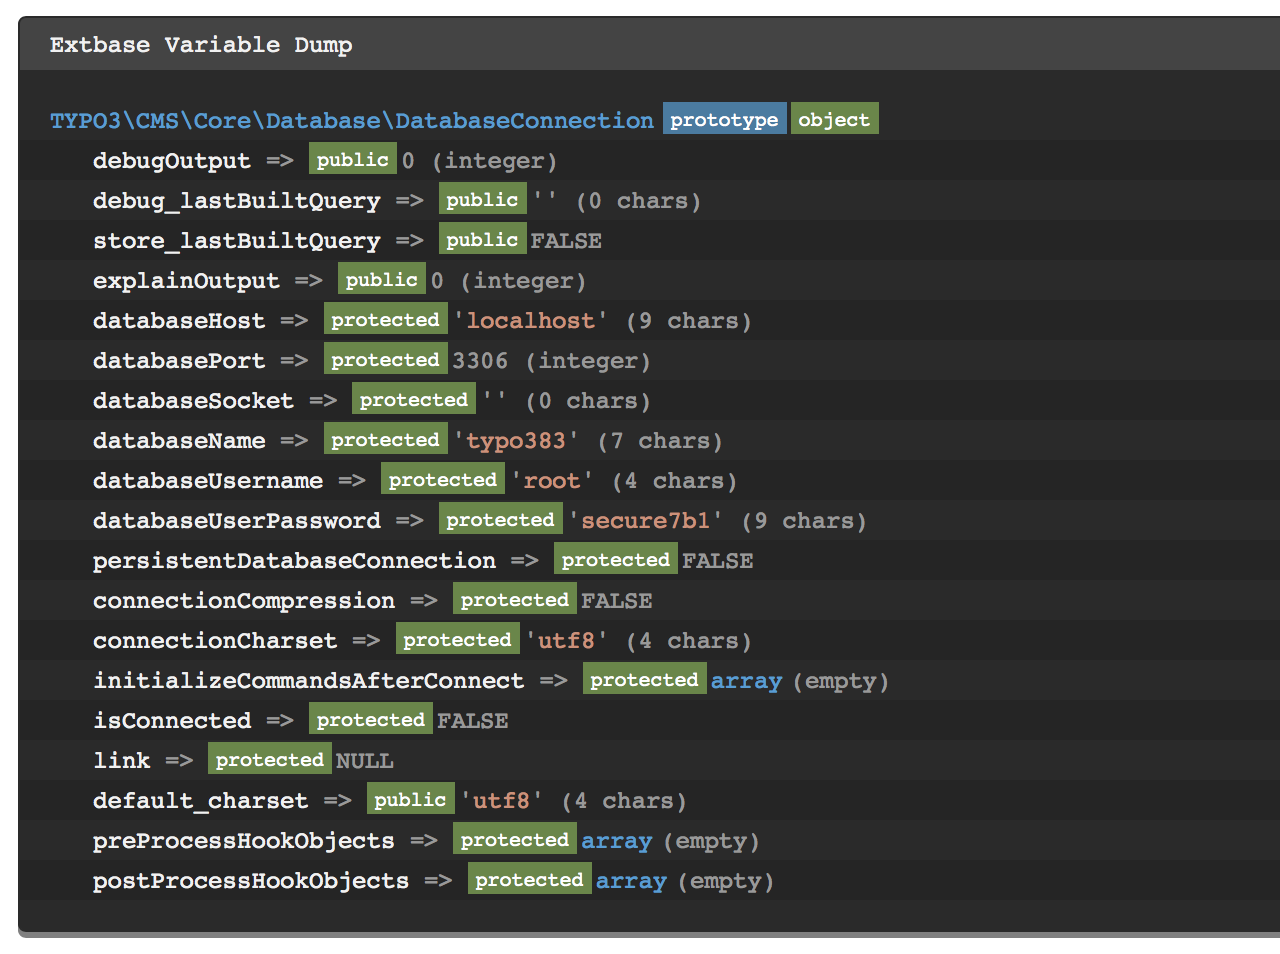
\includegraphics[width=0.65\linewidth]{InDepthChanges/76008.png}
	\end{figure}

\end{frame}

% ------------------------------------------------------------------------------
% LTXE-SLIDE-START
% LTXE-SLIDE-UID:		049acb59-12fc5808-ff0ef982-78a2b57f
% LTXE-SLIDE-ORIGIN:	2b74180d-e68ba0c2-8826a2cf-8498f977 English
% LTXE-SLIDE-TITLE:		!Breaking: #73461 - Import module disabled for non admin users
% LTXE-SLIDE-REFERENCE:	!Breaking-73461-ImportModuleDisabledForNonAdminUsers.rst
% ------------------------------------------------------------------------------
\begin{frame}[fragile]
	\frametitle{Cambios en Profundidad}
	\framesubtitle{Módulo de Importación Deshabilitado para Usuarios no Administradores}

	\begin{itemize}

		\item El módulo de importación de \texttt{EXT:impexp} está ahora deshabilitado para usuarios no-administradores por defecto

		\item Para usuarios no-administradores, que necesitan esta funcionalidad, la siguiente opción de Usuario TSconfig
			puede ser configurada:\newline
			\texttt{options.impexp.enableImportForNonAdminUser = 1}

			\vspace{0.5cm}

			\begingroup
				\color{typo3red}
				Advertencia: esto puede llegar a ser un problema de seguridad en las versiones 6.2 y 7.6 de TYPO3
				y debe ser habilitado para usuarios de backend de \textit{confianza}.
			\endgroup

	\end{itemize}

\end{frame}

% ------------------------------------------------------------------------------
% LTXE-SLIDE-START
% LTXE-SLIDE-UID:		1bfba433-558f4508-5fa9fedd-5e0a5b22
% LTXE-SLIDE-ORIGIN:	bac423cc-ba00db30-e1538b7f-25749380 English
% LTXE-SLIDE-TITLE:		Hooks and Signals (1)
% LTXE-SLIDE-REFERENCE:	!Feature-76209-HookToRegisterCustomResultBrowsersInAbstractPlugin.rst
% ------------------------------------------------------------------------------
\begin{frame}[fragile]
	\frametitle{Cambios en Profundidad}
	\framesubtitle{Hooks y Señales (1)}

	% decrease font size for code listing
	\lstset{basicstyle=\tiny\ttfamily}

	\begin{itemize}

		\item Un nuevo hook permite registrar implementaciones de resultados de navegador personalizados

		\item Este enfoque permite sobreescribir la implementación por defecto de
			\texttt{AbstractPlugin::pi\_list\_browseresults()}
			para todas aquellas extensiones o sólo para algunas específicas

		\item El hook puede ser registrado en \texttt{ext\_localconf.php}:

			\begin{lstlisting}
				$GLOBALS['TYPO3_CONF_VARS']['SC_OPTIONS']
				  [\TYPO3\CMS\Frontend\Plugin\AbstractPlugin::class]['pi_list_browseresults'][1463475262] =
				  \Vendor\ExtensionKey\Hook\ResultBrowserHook::class
			\end{lstlisting}

	\end{itemize}

\end{frame}


% ------------------------------------------------------------------------------
% LTXE-SLIDE-START
% LTXE-SLIDE-UID:		2bc560ee-4c416fbe-d902f8bf-ee5d462a
% LTXE-SLIDE-ORIGIN:	82c70aee-3b375252-6cac0ad6-b385b95f English
% LTXE-SLIDE-TITLE:		Hooks and Signals (2)
% LTXE-SLIDE-REFERENCE:	!Feature-76259-IntroduceBuildQueryParametersPostProcessHook.rst
% ------------------------------------------------------------------------------
\begin{frame}[fragile]
	\frametitle{Cambios en Profundidad}
	\framesubtitle{Hooks y Señales (2)}

	% decrease font size for code listing
	\lstset{basicstyle=\tiny\ttfamily}

	\begin{itemize}

		\item Con la migración a Doctrine, el hook \texttt{buildQueryParameters} ha sido introducido en la clase
			\texttt{DatabaseRecordList}.

		\item Este hook reemplaza el hook \texttt{makeQueryArray} del método obsoleto
			\texttt{AbstractDatabaseRecordList::makeQueryArray}.

		\item El uso del nuevo hook permite modificar los parámetros usados para consultar la base de datos de registros
			a ser mostrados en la vista de lista de registros

		\item El hook puede ser registrado en \texttt{ext\_localconf.php}:

			\begin{lstlisting}
				$GLOBALS['TYPO3_CONF_VARS']['SC_OPTIONS']
				  [\TYPO3\CMS\Recordlist\RecordList\DatabaseRecordList::class]['buildQueryParameters'][]
			\end{lstlisting}

		\item ...e implementa el método público \texttt{buildQueryParametersPostProcess}

	\end{itemize}

\end{frame}

% ------------------------------------------------------------------------------
% LTXE-SLIDE-START
% LTXE-SLIDE-UID:		ae3a6158-03ec9d29-cc4ac8ea-d96ae870
% LTXE-SLIDE-ORIGIN:	73d888ce-a14c0f6a-d4dec5fb-f7368bb6 English
% LTXE-SLIDE-TITLE:		!Breaking: #76108 - Replace ExtJS category tree with D3 and SVG
% LTXE-SLIDE-TITLE:		!Feature: #77349 - Additional locations for extension icons
% LTXE-SLIDE-TITLE:		!Feature: #77481 - Add possibility to define a favicon for the backend
% LTXE-SLIDE-REFERENCE:	!Breaking-76108-ReplaceExtJSCategoryTreeWithD3AndSVG.rst
% LTXE-SLIDE-REFERENCE:	!Feature-77349-AdditionalLocationsForExtensionIcons.rst
% LTXE-SLIDE-REFERENCE:	!Feature-77481-AddPossibilityToDefineAFaviconForTheBackend.rst
% ------------------------------------------------------------------------------
\begin{frame}[fragile]
	\frametitle{Cambios en Profundidad}
	\framesubtitle{Miscelánea}

	\begin{itemize}

		\item Renderizado de SVGs y D3

			\begin{itemize}
				\item Como parte de la eliminación de ExtJS del código de TYPO3, el árbol dentro de la edición de formulario ha sido rediseñado
				\item El renderizado está basado en SVGs y D3 ahora, lo que viene con una mejora significante de rendimiento
				\item El rediseño del árbol de páginas del mismo está planeado para el futuro cercano
			\end{itemize}

		\item Iconos de extensiones pueden ser almacenados en el siguiente directorio ahora:\newline
			\small
				\texttt{Resources/Public/Icons/<nombre de fichero>}
				(donde <nombre de fichero> puede ser: \texttt{Extension.png}, \texttt{Extension.svg} o \texttt{Extension.gif})
			\normalsize

		\item La nueva opción \texttt{backendFavicon} en la configuración del Manejador de Extensiones hace posible
			cambiar el favicon del backend.

	\end{itemize}

\end{frame}

% ------------------------------------------------------------------------------
